\documentclass[10pt,twocolumn]{article}

\usepackage[letterpaper,margin=0.72in,columnsep=0.25in]{geometry}
\usepackage[T1]{fontenc}
\usepackage{lmodern}
\usepackage{microtype}
\usepackage{booktabs}
\usepackage{tabularx}
\usepackage{multirow}
\usepackage{siunitx}
\usepackage{xcolor}
\usepackage{graphicx}
\usepackage{pgfplots}
\usepackage{enumitem}
\usepackage{hyperref}

\pgfplotsset{compat=1.18}
\sisetup{detect-all,group-separator={,},group-minimum-digits=4}
\setlist{leftmargin=*,nosep}
\setlength{\emergencystretch}{1.5em}

\definecolor{cpu}{HTML}{4C78A8}
\definecolor{scanline}{HTML}{F58518}
\definecolor{direct}{HTML}{54A24B}
\definecolor{turbo}{HTML}{E45756}
\definecolor{imageio}{HTML}{B279A2}

\hypersetup{
  colorlinks=true,
  linkcolor=cpu,
  citecolor=direct,
  urlcolor=cpu,
  pdftitle={Characterizing Single-Image JPEG Decode on Apple Silicon},
  pdfauthor={Adam DePrince}
}

\newcommand{\system}{JPEGli--Metal}
\newcommand{\cpu}{CPU JPEGli}
\newcommand{\direct}{direct Metal}
\newcommand{\scanline}{Metal-to-CPU}
\newcommand{\code}[1]{\texttt{#1}}
\newcommand{\percent}[1]{#1\%}
\newcommand{\mib}{\,MiB}

\title{Characterizing Single-Image JPEG Decode on Apple Silicon:\\
       A Direct-Metal Reconstruction Backend for JPEGli}
\author{Adam DePrince}
\date{August 2026}

\begin{document}
\maketitle

\begin{abstract}
Consumer image decode is a latency-sensitive heterogeneous workload: the
serial entropy front end is difficult to parallelize, while inverse transform,
upsampling, and color conversion expose abundant data parallelism.  This paper
presents and characterizes an experimental direct-Metal reconstruction backend
for JPEGli on Apple M4.  Marker parsing, Huffman decoding, restart/EOB state,
and progressive scan processing remain on one CPU thread.  Quantized
coefficient planes are produced directly in unified memory; Metal performs
adaptive dequantization, 8$\times$8 IDCT, chroma reconstruction, color
conversion, and RGBA8 output.  The implementation preserves the libjpeg API,
adds GPU-native output endpoints, and falls back to the CPU for unsupported
modes.

On 30 CLIC 2025 images, warm direct-texture latency at quality-90 4:2:0 falls
from 9.571 to 4.476 ms for baseline JPEG and from 18.982 to 14.065 ms for
progressive JPEG.  A conservative 480,000-pixel policy is faster at both p50
and p95 across the tested quality, sampling, and scan configurations.  The
direct path uses 25.02 MiB median retained memory for 4:2:0 and is byte-for-byte
identical to CPU JPEGli.  That exactness retains JPEGli's distinct perceptual
behavior: in a four-metric Q25--100 sweep, Q100 JPEGli lowers all four
aggregate distortions relative to TurboJPEG at 4:4:4, 4:2:2, and 4:2:0,
although DISTS favors both incumbents through Q95.  Across a separate
1,500-window campaign, direct Metal consumes
53.8\% less \emph{process-attributed} energy than CPU JPEGli and is effectively
tied with TurboJPEG overall (0.3\% less), while using 27.1\% less than
TurboJPEG on large baseline images.  The macOS counter is not whole-device
energy; consequently, we do not claim a battery-energy ranking against
ImageIO.  The results show that final reconstruction is a useful GPU boundary
for substantial baseline images, but that small and progressive inputs remain
limited by submission overhead and serial CPU work.
\end{abstract}

\section{Introduction}

JPEG decode separates naturally into two unlike phases.  Parsing and Huffman
entropy decode are stateful and branch-heavy, whereas dequantization, inverse
DCT, chroma upsampling, and color conversion apply regular operations over
many 8$\times$8 blocks~\cite{wallace1992jpeg}.  Desktop decoders such as
libjpeg-turbo accelerate the latter operations with CPU SIMD
instructions~\cite{libjpegturbo}.  Apple silicon adds a tightly integrated GPU
and a shared storage mode in which the CPU and GPU access one system-memory
allocation~\cite{apple-shared-storage}.  That organization invites a narrower
question than generic ``GPU JPEG decode'': can the final reconstruction phase
be moved to Metal without damaging one-image responsiveness?

This work targets an interactive consumer application decoding one image for
immediate use.  It therefore deliberately excludes batching, pipelining,
worker pools, multiple command streams, and concurrent decoder jobs.  Those
techniques can amortize GPU overhead in servers but change the latency and
memory problem faced by a photo viewer, browser, or UI.

JPEGli is an interesting base for this experiment because its decoder performs
floating-point reconstruction and expectation-based adaptive dequantization,
rather than simply reproducing a conventional integer reconstruction
pipeline~\cite{jpegli}.  A GPU implementation must match that behavior exactly
if it is to remain behind an existing libjpeg-compatible API.

The practical rationale is also perceptual.  Replacing CPU JPEGli with a
faster conventional decoder changes pixels reconstructed from the same JPEGli
bitstream.  Our quality study finds that JPEGli's reconstruction becomes
increasingly favorable at high quality, but also exposes meaningful metric
disagreement.  At Q95, SSIMULACRA2, Butteraugli, and ColorVideoVDP generally
favor JPEGli while DISTS favors the incumbents; at Q100 JPEGli leads
TurboJPEG on all four aggregate metrics in every sampling mode.  Metal
acceleration can therefore close the performance gap while retaining the
selected reconstruction behavior; an approximate GPU kernel would change the
very output being evaluated.

This paper makes four contributions:

\begin{itemize}
  \item a direct Objective-C++/Metal backend that retains JPEG parsing and
        progressive scan state on the CPU, but reconstructs completed
        coefficient planes on the GPU;
  \item a zero-coefficient-copy unified-memory path, fused sampling-specific
        kernels, a direct texture API, bounded resource retention, and an
        empirical CPU/GPU crossover policy;
  \item exact-output and compatibility validation across baseline,
        progressive, grayscale, RGB/YCbCr, 4:4:4, 4:2:2, 4:2:0, odd-size,
        restart, suspension, fallback, malformed-input, abort, and destroy
        cases; and
  \item a single-image characterization of warm and cold latency, stage time,
        memory, perceptual behavior, and process-attributed energy on an Apple
        M4 Max.
\end{itemize}

The central result is conditional rather than universal.  Direct Metal is a
large win for substantial baseline images, reaches a smaller win after a
progressive CPU front end, and loses to TurboJPEG for most small inputs.  An
explicit crossover and output-aware policy are therefore part of the system,
not an afterthought.

\section{System Design}
\label{sec:design}

\subsection{CPU/GPU boundary}

The CPU retains JPEG marker parsing, Huffman/entropy decoding, restart marker
handling, EOB state, coefficient refinement, and progressive scan state.  It
produces the same quantized coefficient planes needed by the existing CPU
renderer.  Once all required scans are decoded, Metal performs adaptive
dequantization, 8$\times$8 IDCT, chroma upsampling, YCbCr-to-RGB conversion,
and RGBA8 output.  RGB JPEG and grayscale inputs use corresponding specialized
paths.  Incremental buffered progressive display remains on the CPU because a
partially reconstructed image has different semantics from a completed
single-image result.

The boundary was selected to keep complex, serial bitstream state in the
mature decoder and offload the regular portion.  Entropy decode remains the
critical limit for progressive images, a fact borne out in
Section~\ref{sec:stages}.

\subsection{Unified coefficient storage}

When an input is eligible, entropy decode writes coefficient blocks directly
to an \code{MTLStorageModeShared} buffer.  The CPU and GPU therefore see the
same allocation, consistent with Metal's shared-storage semantics on Apple
silicon~\cite{apple-shared-storage,apple-unified-memory}.  There is no second
full coefficient-image copy.  Per-iMCU adaptive-dequantization statistics are
updated as coefficients arrive, including progressive refinement and input
rollback, eliminating a later analysis sweep.

JPEGli stores blocks in natural coefficient order, so this implementation does
not require a separate inverse-zigzag kernel.  A decoder with zigzag-ordered
planes would place reordering at this reconstruction boundary rather than
altering entropy state.

\subsection{Fused kernels}

Pipelines are specialized by sampling mode.  Grayscale, 4:4:4, and
box-filtered 4:2:2/4:2:0 combine dequantization, IDCT, sampling, color
conversion, and output in one tiled kernel.  Fancy 4:2:2/4:2:0 first
reconstructs the two smaller chroma planes, then fuses luma IDCT, chroma
sampling, color conversion, and output.  Consequently, 4:4:4 retains no
full-resolution floating-point component planes.  IDCT rows and columns are
evaluated cooperatively by SIMD-group lanes with a threadgroup transpose; all
work for one image is encoded into one command buffer.  This follows Metal's
basic work-submission model while minimizing CPU commands on the critical
path~\cite{apple-metal-calculation,apple-command-structure}.

The shaders use precise floating-point compilation and match the CPU
constants and operation ordering.  Exact pixel tests, rather than a tolerance,
are the acceptance criterion.  Unsupported modes fall back instead of
quietly accepting floating-point drift.

\subsection{Output and lifecycle}

Three GPU-visible completion choices are exposed:

\begin{enumerate}
  \item the existing scanline API, which waits for Metal and copies RGBA rows
        to caller memory;
  \item an owned shared buffer plus RGBA8Unorm texture view, completed before
        return; and
  \item a caller-owned command buffer and texture, into which JPEGli encodes
        without committing or waiting.
\end{enumerate}

The last endpoint lets an application put display or Core Image work in the
same command buffer.  It also makes the semantic difference between CPU and
GPU consumers explicit: a direct texture is complete output, not an omitted
copy from an otherwise CPU-visible result.

Device, queue, precompiled shader library, and pipeline states are initialized
lazily.  Retaining pipeline state avoids moving driver compilation onto every
decode; Apple similarly recommends creating expensive pipeline objects away
from time-critical work~\cite{apple-pipeline-state}.  One scratch set is
cached.  Sets larger than 96 MiB are released, a predicted Metal working set
above 512 MiB falls back before allocation, and exported output is never part
of the scratch cache.  Public release calls discard scratch alone or the full
inactive context under memory pressure.  Output objects independently retain
resources required after decoder destruction.

\subsection{Eligibility and compatibility}

The backend is guarded by \code{JPEGLI\_ENABLE\_APPLE\_METAL}, disabled by
default, and compiled only on Apple platforms.  The installed capability and
policy API is still present in Metal-disabled builds, where availability is
false and normal decode stays on the CPU.  Standard scanline decoding uses an
AUTO policy.  FORCE and direct-texture requests bypass the size threshold but
not correctness, device, format, or working-set checks.

Full-scale 8-bit RGBA output from grayscale, RGB, and YCbCr baseline or
progressive JPEG is eligible for common 4:4:4, 4:2:2, and 4:2:0 ratios.
Scaled IDCT, raw output, color quantization, CMYK/YCCK, unusual ratios, and
buffered incremental output transparently retain the CPU renderer.  A
caller-command request returns failure rather than silently targeting another
texture; the ordinary CPU decoder remains usable.

\section{Experimental Method}
\label{sec:method}

\subsection{Platform and builds}

Experiments ran on a Mac16,5 with an Apple M4 Max, 12 performance and 4
efficiency CPU cores, a 40-core GPU, 128 GiB unified memory, and macOS 26.5.1
(build 25F80).  The machine was connected to AC power in High Power Mode, and
the campaign recorded no thermal or performance warning.  Metal-enabled and
Metal-disabled Release trees were built independently.  A full Xcode Metal
toolchain embedded a precompiled \code{metallib}; the runtime compiler
fallback was tested separately but is not the reported fast path.

All work was serial.  A benchmark invocation held at most one image in flight
and created a normal decoder lifecycle for each decode.  Encoding was outside
all timed regions.  Timed output was opaque RGBA8.

\subsection{Latency corpus and protocol}

The primary latency corpus contains the 30 CLIC 2025 test images, between 1.90
and 4.19 megapixels each.  CLIC provides high-resolution photographic and
screen/game material for compression evaluation~\cite{clic2025}.  JPEGli
encoded each source at quality 90 for 4:2:0 and 4:4:4, in both baseline and
progressive form.

Each path received three warmups and 25 measured decodes per image.  Path
order rotated between repetitions.  \emph{Ready} ends when CPU scanlines or a
completed texture can be consumed.  \emph{Total} additionally includes
finish, destroy, and exported-object release.  The caller-command path records
both encoded-return and completed-ready time.  Cold trials release JPEGli's
process-global Metal context before each decode, but do not restart the
process or purge macOS driver caches.

Stage timers separate CPU entropy/coefficient work, Metal initialization,
coefficient analysis/copy, command encoding and submission, GPU kernels,
CPU-output copy, and total reconstruction.  GPU elapsed times use Metal
timestamps when available.  Memory accounting reports decoder allocations and
retained Metal buffers; application-owned destination texture bytes are
excluded from the caller-owned column.

\subsection{Crossover protocol}

A deterministic source image was resampled from 64$\times$64 through
4096$\times$3072.  Sweeps covered qualities 50, 90, and 95; baseline and
progressive coding; and 4:4:4 and 4:2:0.  A boundary was accepted only where
Metal-to-CPU beat the CPU at both p50 and p95 in every final configuration.
This intentionally favors predictable responsiveness over choosing Metal at
the first average win.

\subsection{Decoder and quality comparisons}

CPU JPEGli, TurboJPEG 3.2.0, and Apple ImageIO were measured as incumbent
CPU/framework paths.  Accelerated outputs were compared byte-for-byte with
CPU JPEGli.  Incumbent outputs were checked for successful decode, dimensions,
and opaque RGBA, but not byte equality: JPEGli's expectation-based
dequantization intentionally reconstructs different pixels.

The quality corpus uses all 30 CLIC sources at encoder qualities 25 through
100 in steps of five and at 4:4:4, 4:2:2, and 4:2:0 sampling.  The baseline
scan layout is sufficient here because scan order does not change the final
quantized coefficient set.  Each JPEG is decoded by CPU JPEGli, TurboJPEG,
and ImageIO; ImageIO is drawn explicitly into an sRGB context.  The exact RGB
samples used by the in-process metrics are serialized losslessly for the two
external metrics.

Four full-reference metrics compare each decoded JPEG with its original:
SSIMULACRA2 (higher), Butteraugli (lower), ColorVideoVDP JOD (higher), and
DISTS (lower)~\cite{ssimulacra2,butteraugli,colorvideovdp,dists}.
ColorVideoVDP 0.5.6 uses its \code{standard\_4k} SDR display model.  DISTS
0.1 evaluates native-resolution sRGB tensors without resizing, using its
published weights and ImageNet VGG16 features.  Both learned metrics run in
inference mode through PyTorch/MPS; PyTorch is not part of any decoder path.
Package, model, display-configuration, and input hashes accompany the raw
results.

To put metrics with opposite directions on one plot, we convert each score to
distortion: $100-S$ for SSIMULACRA2, $10-J$ for ColorVideoVDP, and the raw
Butteraugli or DISTS distance.  We first average each decoder's distortion
over the 30 paired images, then divide incumbent distortion by JPEGli
distortion.  Thus values above one consistently favor JPEGli, and a base-2
logarithmic ordinate gives reciprocal ratios equal visual distance.  Averaging
before division remains defined when an individual ColorVideoVDP observation
reaches its 10-JOD ceiling.  Off-scale ratios are labeled rather than silently clipped.
Per-image win counts accompany the aggregate curves.  Since every Metal result
equals CPU JPEGli, it necessarily inherits the same four scores; these metrics
characterize decoder behavior, not a GPU approximation.

\subsection{Energy protocol}
\label{sec:energy-method}

Short per-decode energy deltas were often quantized to zero, so a separate
44-minute campaign used five image classes---screen/UI, standard photograph,
high texture, synthetic edges, and grayscale photograph---at one small and
one large size.  JPEGli encoded six profiles: Q50 4:2:0 baseline; Q90 4:2:0,
4:2:2 baseline; Q95 4:4:4 baseline; and Q90 4:2:0, 4:4:4 progressive.

For every profile, image, and path, three warmups preceded five rotated
measurement windows.  A window repeatedly decoded the \emph{same} image
serially for at least 1.5 s after a 250 ms settle interval.  Repetition only
resolved counter granularity; it did not introduce parallelism or reuse a
decoder across images.  All 1,500 requested windows returned an energy value
and no sample was removed.

The counter is the delta of macOS
\nolinkurl{RUSAGE_INFO_V6.ri_energy_nj} for the benchmark process.  We report it
as \emph{process-attributed energy}; average attributed watts divide that
delta by wall time.  This is not battery, adapter, or rail telemetry.  Work in
an Apple framework, driver, hardware block, or service need not be billed
fully to the caller.  The limitation is conspicuous for large ImageIO cases,
so ImageIO numbers are shown but never interpreted as a whole-device ranking.

For each image/path case, tables use the median of five trials.  Aggregate
ratios are paired geometric means, giving each image/profile case equal
weight.  Negative deltas mean less time or attributed energy.

\section{Latency Results}
\label{sec:latency}

\begin{figure*}[t]
  \centering
  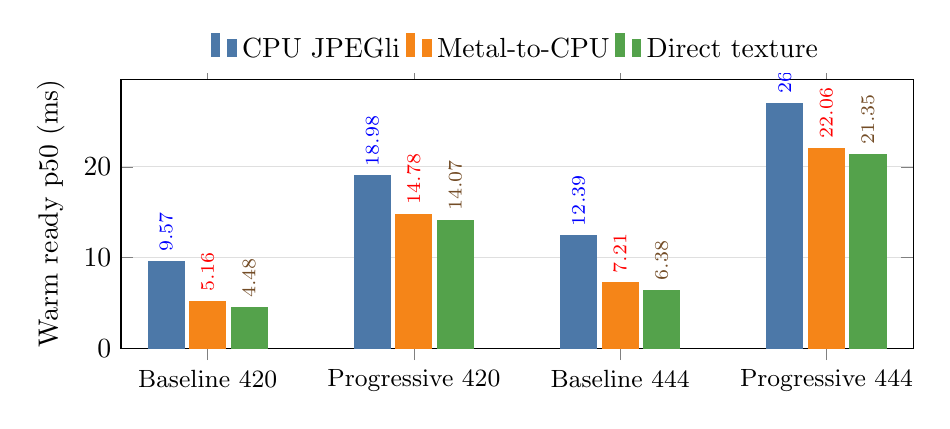
\begin{tikzpicture}
    \begin{axis}[
      width=0.96\textwidth,
      height=5.0cm,
      ybar=2pt,
      bar width=13pt,
      ymin=0,
      ylabel={Warm ready p50 (ms)},
      symbolic x coords={Baseline 420,Progressive 420,Baseline 444,Progressive 444},
      xtick=data,
      x tick label style={font=\small},
      ymajorgrids=true,
      grid style={draw=gray!25},
      legend style={at={(0.5,1.02)},anchor=south,legend columns=3,draw=none},
      nodes near coords,
      nodes near coords style={font=\scriptsize,rotate=90,anchor=west},
      enlarge x limits=0.14,
    ]
      \addplot+[fill=cpu,draw=cpu] coordinates {
        (Baseline 420,9.571) (Progressive 420,18.982)
        (Baseline 444,12.393) (Progressive 444,26.963)};
      \addplot+[fill=scanline,draw=scanline] coordinates {
        (Baseline 420,5.158) (Progressive 420,14.779)
        (Baseline 444,7.205) (Progressive 444,22.061)};
      \addplot+[fill=direct,draw=direct] coordinates {
        (Baseline 420,4.476) (Progressive 420,14.065)
        (Baseline 444,6.381) (Progressive 444,21.354)};
      \legend{CPU JPEGli,Metal-to-CPU,Direct texture}
    \end{axis}
  \end{tikzpicture}
  \caption{Warm single-image readiness on 30 CLIC images (Q90).  Direct output
  removes the final CPU-visible pixel copy.  Progressive entropy and scan
  processing remain on the CPU.}
  \label{fig:warm-latency}
\end{figure*}

\subsection{Warm one-image latency}

Figure~\ref{fig:warm-latency} and Table~\ref{tab:warm} show the primary
result.  For baseline 4:2:0, \scanline{} lowers pooled p50 readiness by 46.1\%
and \direct{} by 53.2\%.  Per-image paired median speedups are 1.772$\times$
and 2.058$\times$, respectively.  The direct path reaches 631.2 MP/s.

Progressive 4:2:0 improves less: 22.1\% for CPU-visible output and 25.9\% for
direct output, with 1.265$\times$ and 1.338$\times$ paired speedups.  More
chroma work in 4:4:4 reduces the absolute throughput of every path, but direct
Metal still reaches 1.887$\times$ paired speedup for baseline and
1.255$\times$ for progressive input.

\begin{table}[t]
  \centering
  \caption{Warm Q90 readiness and direct-path speedup.}
  \label{tab:warm}
  \small
  \begin{tabular}{@{}llrrr@{}}
    \toprule
    Scans & Sampling & CPU & Direct & Speedup \\
          &          & p50 ms & p50 ms & paired \\
    \midrule
    Baseline    & 4:2:0 & 9.571  & 4.476  & 2.058$\times$ \\
    Progressive & 4:2:0 & 18.982 & 14.065 & 1.338$\times$ \\
    Baseline    & 4:4:4 & 12.393 & 6.381  & 1.887$\times$ \\
    Progressive & 4:4:4 & 26.963 & 21.354 & 1.255$\times$ \\
    \bottomrule
  \end{tabular}
\end{table}

The original three-decoder comparison on the same corpus illustrates the CPU
baseline: sums of per-image medians for baseline 4:2:0 were 288.3 ms for CPU
JPEGli, 143.4 ms for TurboJPEG, and 214.4 ms for ImageIO, corresponding to
299.2, 601.6, and 402.2 MP/s.  Those values came from a separate rotated pass,
so the strongest conclusions use same-pass CPU/Metal pairs and the joint
energy campaign in Section~\ref{sec:energy} rather than treating cross-run
differences as paired observations.

\subsection{Cold start}

Table~\ref{tab:cold} uses the strict library-level cold definition: JPEGli's
global Metal state is released before every image.  Baseline direct readiness
still improves by 17.8\%, but progressive direct improves only 6.6\% because
pipeline setup and serial scans consume most of the available gain.  Median
Metal initialization is 0.28--0.40 ms with the embedded library.  The largest
initialization observed in the 30-image archive pass is 4.927 ms.  Because
driver and process caches remain warm, these numbers are not equivalent to
first launch after boot.

\begin{table}[t]
  \centering
  \caption{Cold Q90 4:2:0 ready latency (ms).}
  \label{tab:cold}
  \small
  \resizebox{\columnwidth}{!}{%
  \begin{tabular}{@{}lrrrr@{}}
    \toprule
    Scans & CPU p50 & Scan p50 & Direct p50 & Direct p95 \\
    \midrule
    Baseline    & 9.639  & 8.444  & 7.928  & 10.912 \\
    Progressive & 18.582 & 17.984 & 17.350 & 26.990 \\
    \bottomrule
  \end{tabular}}
\end{table}

\subsection{Where time goes}
\label{sec:stages}

Table~\ref{tab:stages} reports median warm stages for the 4:2:0
Metal-to-CPU path.  Baseline entropy/coefficient work is 3.192 ms, while
complete Metal reconstruction is 1.248 ms and the requested CPU copy is
0.588 ms.  Moving pixels directly to a GPU consumer removes the last term.

Progressive CPU entropy and scan processing grows to 12.792 ms while GPU work
is almost unchanged.  Amdahl's law therefore predicts, and the end-to-end
measurements confirm, a smaller progressive speedup.  The 4:4:4 fully fused
kernel takes 0.967 ms baseline and 0.966 ms progressive; its complete
reconstruction is 1.740 and 1.812 ms.  These stage values are medians of
independently observed fields and should not be arithmetically summed as if
they came from one synthetic decode.

\begin{table}[t]
  \centering
  \caption{Warm 4:2:0 Metal-to-CPU stages (median ms).}
  \label{tab:stages}
  \small
  \begin{tabular}{@{}lrr@{}}
    \toprule
    Stage & Baseline & Progressive \\
    \midrule
    CPU entropy/coefficient decode & 3.192 & 12.792 \\
    Final bias preparation         & 0.010 & 0.011 \\
    Coefficient copy               & 0.000 & 0.000 \\
    Metal command encoding         & 0.006 & 0.013 \\
    Submission/wait overhead       & 0.462 & 0.497 \\
    Chroma dequantization + IDCT   & 0.195 & 0.194 \\
    Fused luma/sample/color/output & 0.546 & 0.546 \\
    Complete Metal reconstruction  & 1.248 & 1.308 \\
    Requested CPU pixel copy       & 0.588 & 0.587 \\
    \bottomrule
  \end{tabular}
\end{table}

The optimized backend also removes work present in an earlier implementation:
a final coefficient sweep, a coefficient copy, and full floating-point planes.
On the same baseline configuration, complete reconstruction falls from 1.614
to 1.248 ms (22.7\%), while Metal-to-CPU/direct end-to-end p50 falls from
5.351/4.670 to 5.158/4.476 ms (3.6\%/4.2\%).

\section{Crossover and Memory}
\label{sec:crossover}

Several measured configurations cross between 110,592 and 307,200 pixels.
By 480,000 pixels, however, Metal-to-CPU is faster at both p50 and p95 in every
final quality/sampling/scan configuration.  AUTO therefore retains CPU JPEGli
below 480,000 output pixels and attempts Metal at or above it.  Direct texture
endpoints bypass the threshold because the caller has explicitly selected a
GPU consumer; eligibility and memory checks still apply.

This threshold is intentionally not the energy-optimal boundary for every
image.  The energy study finds some savings below it, but progressive small
images are 7.3\% slower than CPU JPEGli and TurboJPEG remains faster and
usually lower in attributed energy.  A responsiveness-first policy should not
sacrifice those common small-image cases for an aggregate-energy statistic.

\begin{table}[t]
  \centering
  \caption{Retained decoder memory on CLIC (median / maximum MiB).}
  \label{tab:memory}
  \scriptsize
  \resizebox{\columnwidth}{!}{%
  \begin{tabular}{@{}llrrr@{}}
    \toprule
    Scans & Sampling & CPU & Metal scan/direct & Caller-owned \\
    \midrule
    Baseline    & 4:2:0 & 0.62 / 0.77  & 25.02 / 36.96 & 14.02 / 20.96 \\
    Progressive & 4:2:0 & 8.43 / 12.68 & 25.02 / 36.96 & 14.02 / 20.96 \\
    Baseline    & 4:4:4 & 0.28 / 0.34  & 27.68 / 40.82 & 16.68 / 24.82 \\
    Progressive & 4:4:4 & 16.11 / 24.26& 27.68 / 40.82 & 16.68 / 24.82 \\
    \bottomrule
  \end{tabular}}
\end{table}

Table~\ref{tab:memory} quantifies the cost of the latency gain.  Median 4:2:0
scratch contains 7.97 MiB of shared coefficients and 5.31 MiB of chroma float
planes.  For 4:4:4, coefficients grow to 15.94 MiB but fusion removes float
planes.  The previous Metal decoder retained 43.43 MiB median and 64.77 MiB
maximum on 4:2:0; shared storage and fusion reduce both by about 42\%.

The direct scanline/texture column includes JPEGli's destination.  The
caller-owned column excludes the application-supplied texture and is the more
useful measure when a display stack already owns its render target.  These
figures are higher than baseline CPU JPEGli and motivate the one-set cache,
96 MiB retention cap, explicit memory-pressure release, and 512 MiB
pre-allocation fallback.

\section{Energy Characterization}
\label{sec:energy}

\begin{figure*}[t]
  \centering
  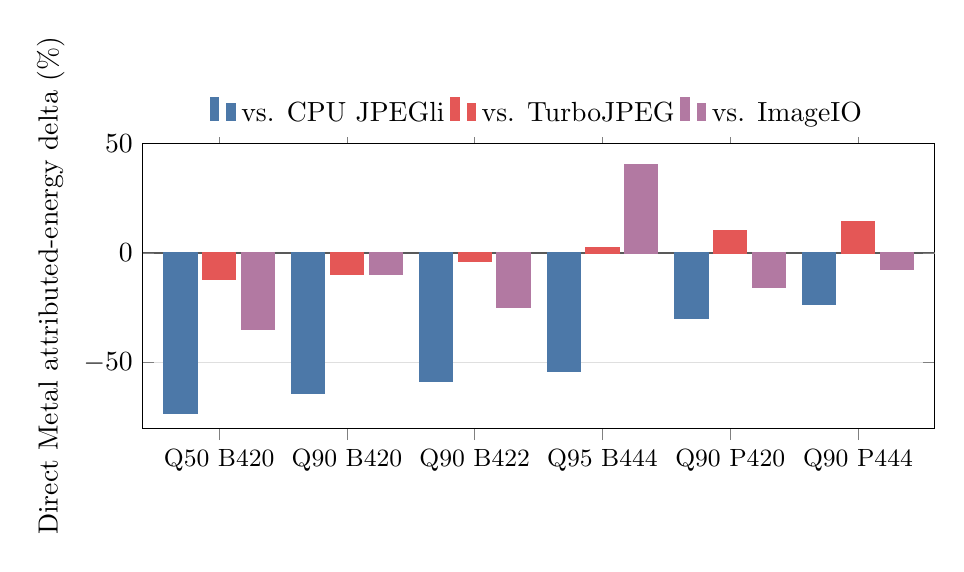
\begin{tikzpicture}
    \begin{axis}[
      width=0.96\textwidth,
      height=5.2cm,
      ybar=2pt,
      bar width=12pt,
      ymin=-80,
      ymax=50,
      ylabel={Direct Metal attributed-energy delta (\%)},
      symbolic x coords={Q50 B420,Q90 B420,Q90 B422,Q95 B444,Q90 P420,Q90 P444},
      xtick=data,
      x tick label style={font=\small},
      ymajorgrids=true,
      grid style={draw=gray!25},
      axis line style={draw=black},
      extra y ticks={0},
      extra y tick labels={},
      extra y tick style={grid=major,grid style={draw=black!65,line width=0.7pt}},
      legend style={at={(0.5,1.02)},anchor=south,legend columns=3,draw=none},
      enlarge x limits=0.12,
    ]
      \addplot+[fill=cpu,draw=cpu] coordinates {
        (Q50 B420,-73.1) (Q90 B420,-64.2) (Q90 B422,-58.7)
        (Q95 B444,-54.2) (Q90 P420,-30.0) (Q90 P444,-23.3)};
      \addplot+[fill=turbo,draw=turbo] coordinates {
        (Q50 B420,-12.1) (Q90 B420,-9.8) (Q90 B422,-3.9)
        (Q95 B444,2.3) (Q90 P420,10.2) (Q90 P444,14.3)};
      \addplot+[fill=imageio,draw=imageio] coordinates {
        (Q50 B420,-34.9) (Q90 B420,-10.0) (Q90 B422,-24.7)
        (Q95 B444,40.2) (Q90 P420,-15.7) (Q90 P444,-7.3)};
      \legend{vs. CPU JPEGli,vs. TurboJPEG,vs. ImageIO}
    \end{axis}
  \end{tikzpicture}
  \caption{Paired geometric-mean process-attributed energy deltas across ten
  images per JPEG profile.  Negative is lower.  ImageIO may execute work that
  is not fully attributed to the client process; its bars are not
  whole-device energy comparisons.}
  \label{fig:energy-profiles}
\end{figure*}

\subsection{Overall and size-dependent results}

Across all 60 image/profile cases, direct Metal uses 53.8\% less attributed
energy than CPU JPEGli, 0.3\% less than TurboJPEG, and 11.4\% less than the
ImageIO client attribution.  Metal-to-CPU uses 47.0\% less than CPU JPEGli but
14.2\% more than TurboJPEG.  Removing readback is therefore material to both
latency and the process counter.

The aggregate tie with TurboJPEG hides a strong size/scan interaction shown in
Table~\ref{tab:energy-groups}.  On large baseline inputs, direct Metal uses
70.2\% less than CPU JPEGli and 27.1\% less than TurboJPEG, winning all 20
paired cases.  On small baseline inputs it still saves 54.7\% relative to CPU
JPEGli but uses 21.1\% more than TurboJPEG.  Progressive CPU work narrows the
large-image gain and makes small direct output 23.7\% more expensive than
TurboJPEG.

\begin{table}[t]
  \centering
  \caption{Direct-Metal paired aggregate deltas.}
  \label{tab:energy-groups}
  \small
  \resizebox{\columnwidth}{!}{%
  \begin{tabular}{@{}lrrr@{}}
    \toprule
    Workload & Energy vs & Energy vs & Latency vs \\
             & CPU JPEGli & TurboJPEG & CPU JPEGli \\
    \midrule
    All 60             & -53.8\% & -0.3\% & -28.3\% \\
    Baseline, small    & -54.7\% & +21.1\%& -10.9\% \\
    Baseline, large    & -70.2\% & -27.1\%& -54.6\% \\
    Progressive, small & -21.3\% & +23.7\%& +7.3\% \\
    Progressive, large & -31.8\% & +1.8\% & -22.2\% \\
    \bottomrule
  \end{tabular}}
\end{table}

Direct Metal beats TurboJPEG in 25 of 60 cases overall; 20 are the large
baseline cases.  Metal-to-CPU wins 19 of those 20.  Both Metal outputs consume
less attributed energy than CPU JPEGli in every case.  Figure
\ref{fig:energy-profiles} further shows that low-quality 4:2:0---where
reconstruction is a larger share of decode---is the best offload case.  Higher
quality, 4:4:4, and progressive scans shift work back to the CPU front end.

The geometric mean of case-median attributed power is 7.15 W for CPU JPEGli,
6.51 W for TurboJPEG, 4.31 W for ImageIO, 4.74 W for Metal-to-CPU, and 4.61 W
for direct Metal.  Energy per image remains the appropriate comparison because
paths run for different durations.  ImageIO's unusually low 0.8--3.6 W client
attribution on several large baseline cases reinforces the limitation from
Section~\ref{sec:energy-method}; it does not establish that the whole Mac used
less power.

\subsection{Repeatability}

Median within-case energy coefficients of variation are 0.81\% for CPU
JPEGli, 0.92\% for TurboJPEG, 0.96\% for ImageIO, 0.71\% for Metal-to-CPU, and
0.90\% for direct Metal.  The 95th-percentile CV is 11.3\% for ImageIO and
1.9--2.4\% for the other paths.  One direct-Metal small-image trial contains
an isolated latency interruption; it remains in the raw data and does not
alter the five-trial median.

\section{Correctness and Visual Quality}
\label{sec:correctness}

The Metal-enabled focused suite passes 16 tests with one expected
unavailable-path skip.  The Metal-disabled configuration passes four
CPU/stub tests and records 13 expected Metal-unavailable skips.  Public API
smoke programs compile against installed headers and link against both fresh
installs.  Static-library symbol audits confirm that the policy, statistics,
direct-output, caller-command, cleanup, and capability interfaces are exported
in both configurations.

Test images cover baseline and progressive scans; qualities 50, 90, and 95;
4:4:4, 4:2:2, and 4:2:0; grayscale, RGB, and YCbCr JPEG; fancy and box
upsampling; odd dimensions; restart intervals; scaled and cropped output;
stream suspension; malformed headers; truncated entropy; buffered progressive
fallback; abort/destroy; and resource release.  Supported Metal cases must be
byte-identical.  Unsupported modes either produce the exact CPU result or, for
the explicit caller-owned endpoint, fail without corrupting subsequent CPU
decode.  The measured 1,500-window matrix records no forced-Metal fallback,
decode error, dimensional mismatch, alpha error, or unavailable energy sample.

\begin{table}[t]
  \centering
  \caption{Number of aggregate perceptual metrics favoring JPEGli out of
  SSIMULACRA2, Butteraugli, ColorVideoVDP, and DISTS.}
  \label{tab:quality}
  \scriptsize
  \begin{tabular}{@{}llccc@{}}
    \toprule
    Incumbent & Sampling & Q90 & Q95 & Q100 \\
    \midrule
    TurboJPEG & 4:4:4 & 3/4 & 3/4 & 4/4 \\
              & 4:2:2 & 3/4 & 3/4 & 4/4 \\
              & 4:2:0 & 2/4 & 3/4 & 4/4 \\
    ImageIO   & 4:4:4 & 3/4 & 3/4 & 4/4 \\
              & 4:2:2 & 3/4 & 3/4 & 4/4 \\
              & 4:2:0 & 2/4 & 3/4 & 3/4 \\
    \bottomrule
  \end{tabular}
\end{table}

\begin{figure*}[t]
  \centering
  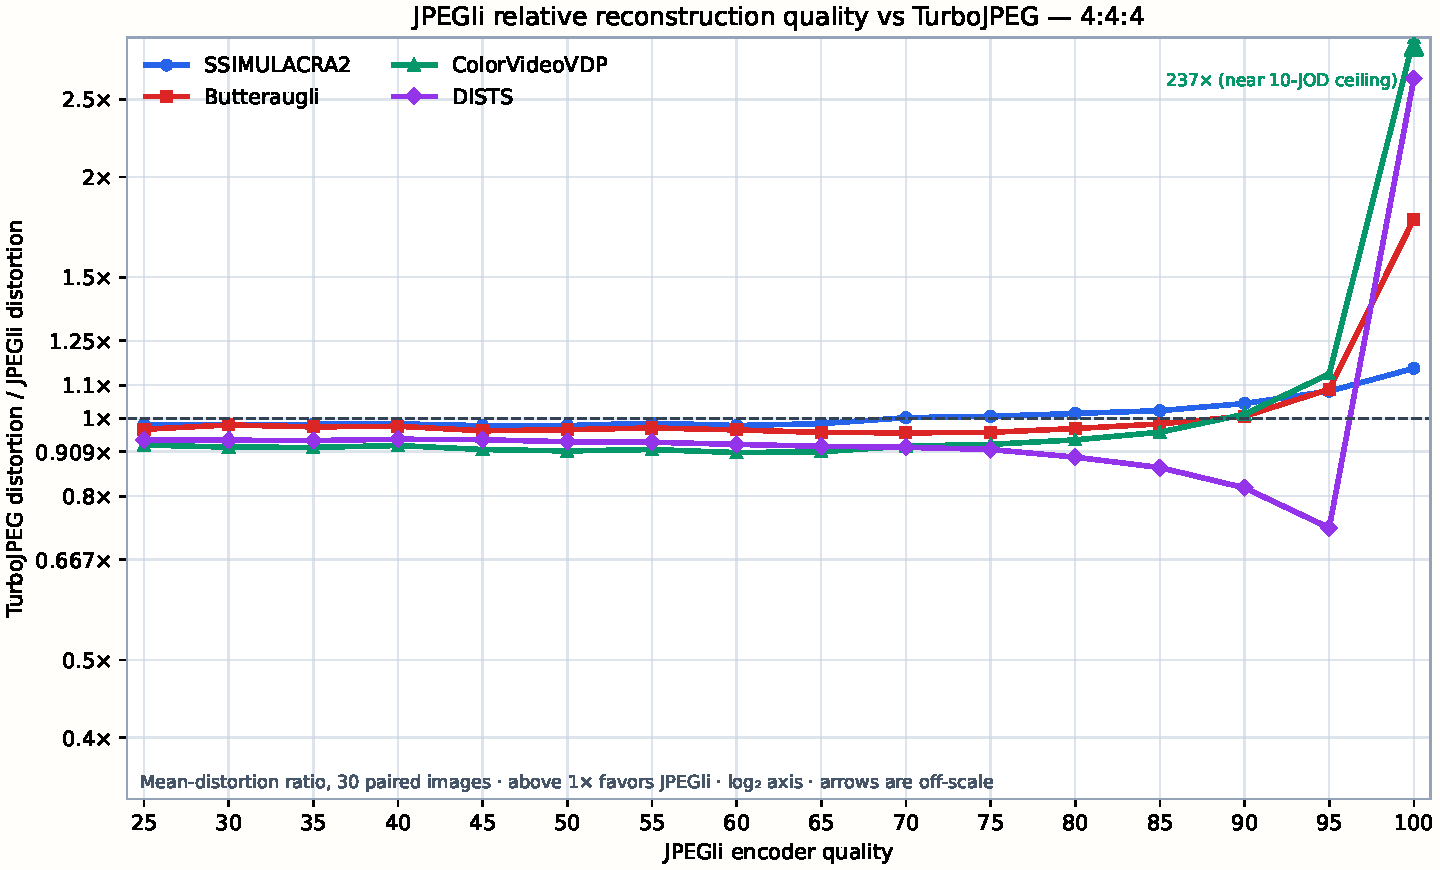
\includegraphics[width=0.49\textwidth]{../perceptual_quality/quality-ratio-turbojpeg-444.pdf}
  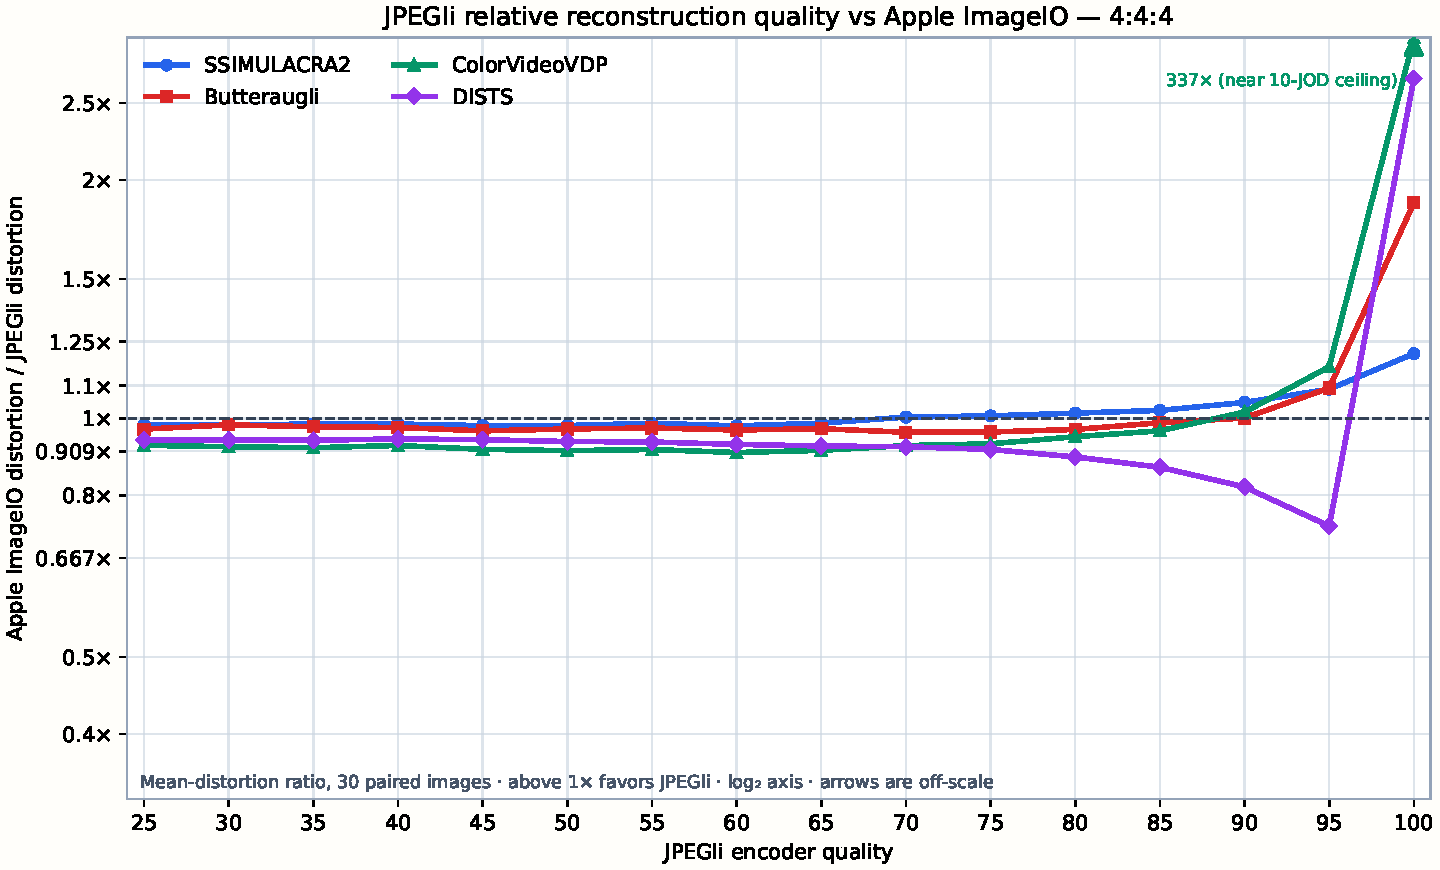
\includegraphics[width=0.49\textwidth]{../perceptual_quality/quality-ratio-apple_imageio-444.pdf}\\
  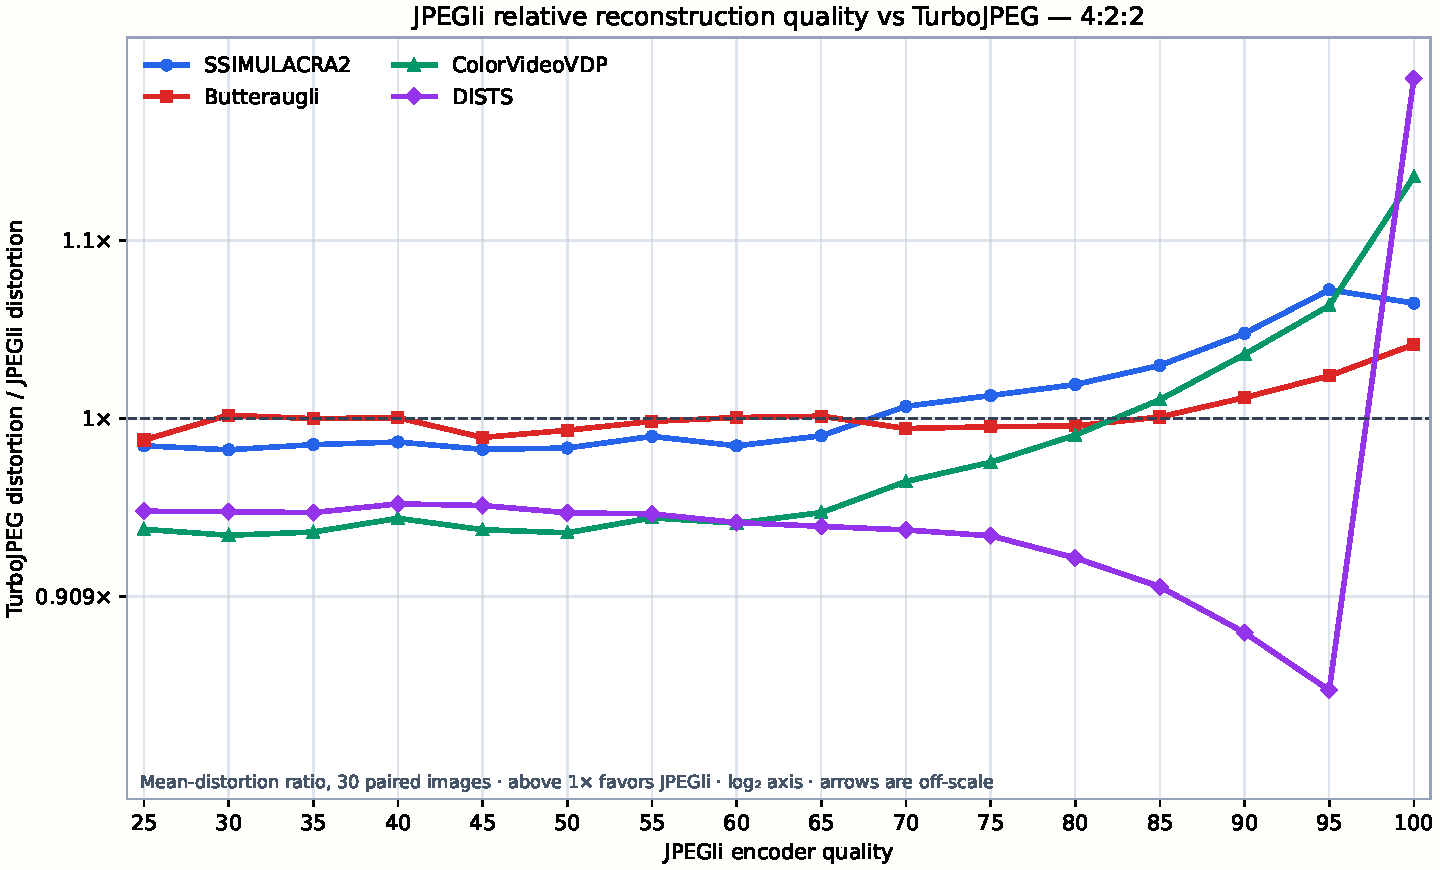
\includegraphics[width=0.49\textwidth]{../perceptual_quality/quality-ratio-turbojpeg-422.pdf}
  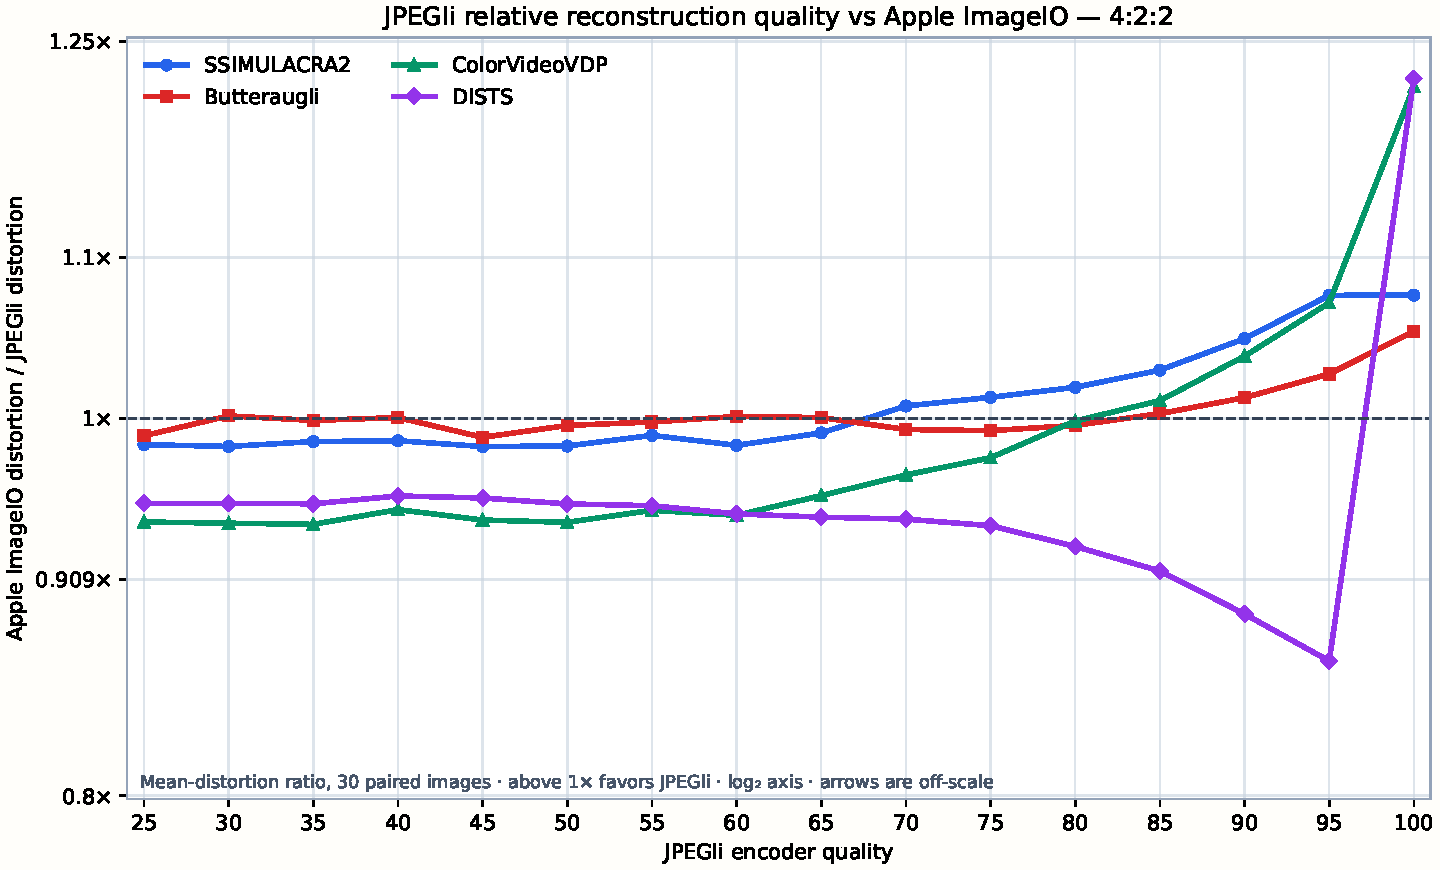
\includegraphics[width=0.49\textwidth]{../perceptual_quality/quality-ratio-apple_imageio-422.pdf}\\
  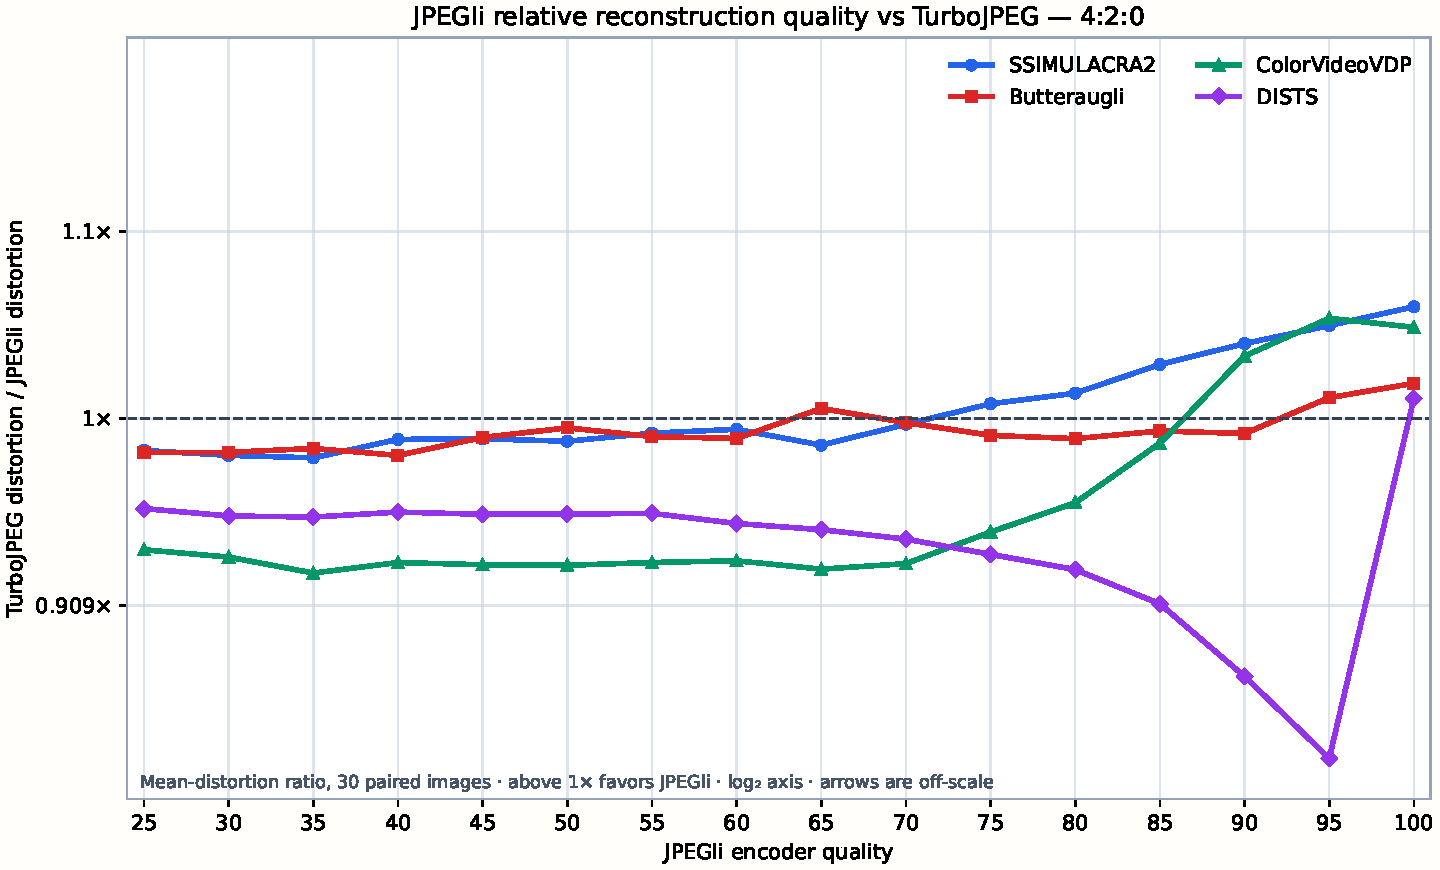
\includegraphics[width=0.49\textwidth]{../perceptual_quality/quality-ratio-turbojpeg-420.pdf}
  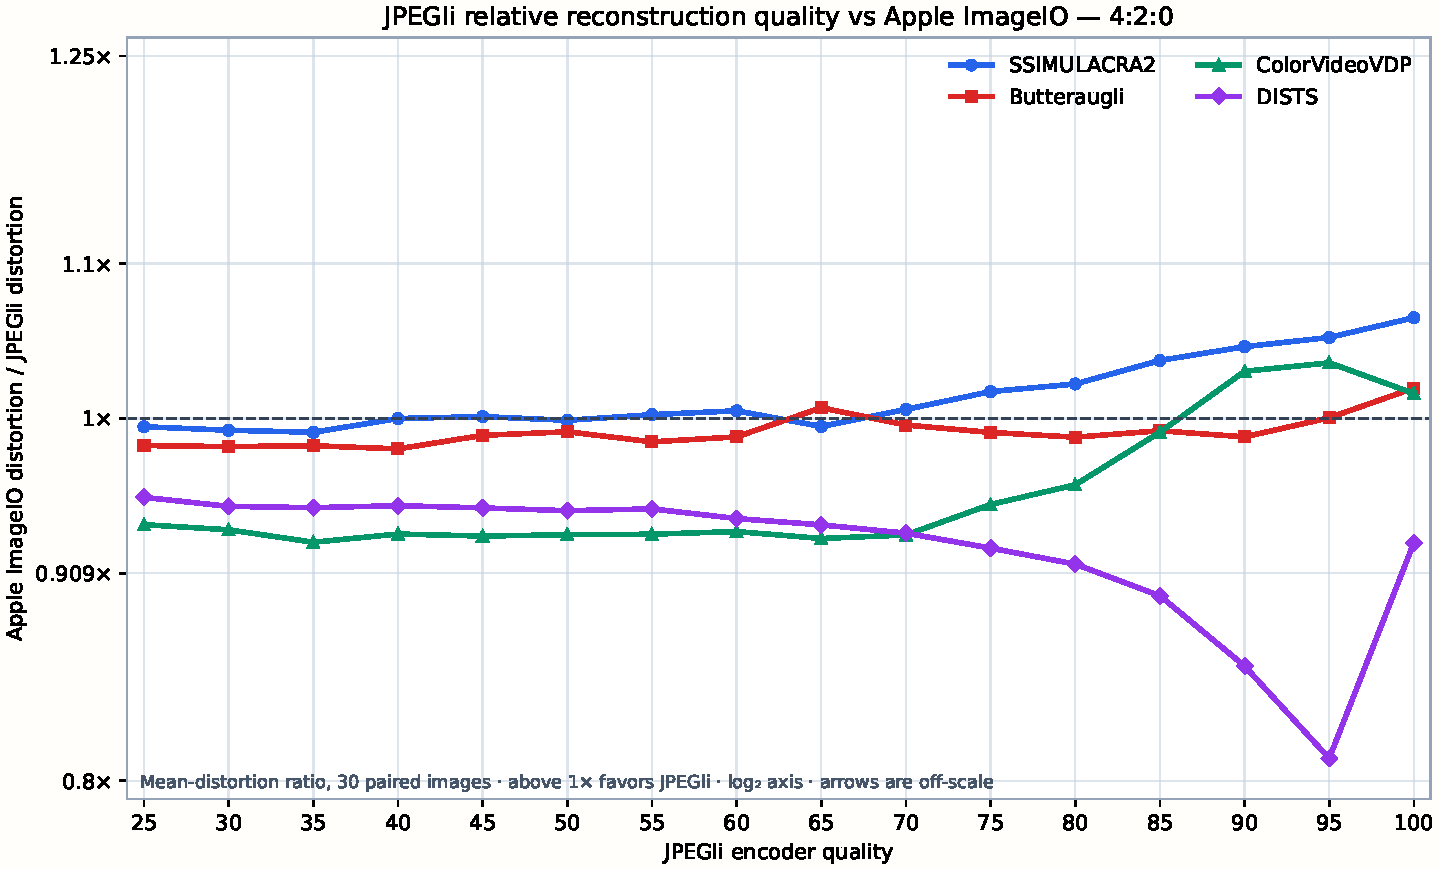
\includegraphics[width=0.49\textwidth]{../perceptual_quality/quality-ratio-apple_imageio-420.pdf}
  \caption{Incumbent mean distortion divided by JPEGli mean distortion over
  30 paired images.  Values above one favor JPEGli.  The base-2 logarithmic
  ordinate makes reciprocal ratios symmetric; labeled arrows are off-scale.}
  \label{fig:quality-ratios}
\end{figure*}

Table~\ref{tab:quality} and Figure~\ref{fig:quality-ratios} confirm that
decoder choice changes perceptual predictions even when the compressed bytes
are fixed, but they do not produce a universal ranking.  At Q90 and Q95,
JPEGli leads three of four metrics for 4:4:4 and 4:2:2; DISTS favors both
incumbents through Q95 in every sampling mode.  At Q100, JPEGli leads
TurboJPEG on all four aggregate metrics for all three sampling modes and
ImageIO on all four for 4:4:4 and 4:2:2.  ImageIO retains a Q100 4:2:0 DISTS
advantage.

Aggregate wins are not per-image guarantees.  Strict all-four Q100 wins are
22/30, 13/30, and 6/30 images against TurboJPEG, and 23/30, 17/30, and 1/30
against ImageIO, for 4:4:4, 4:2:2, and 4:2:0 respectively.  The complete raw
corpus, component mean distortions, and per-image win counts accompany the
paper.

These findings supply an additional rationale for the project.  CPU JPEGli
does not beat TurboJPEG on latency, so a performance-only application could
simply switch decoders.  The Metal backend instead preserves JPEGli's distinct
high-quality reconstruction while recovering or exceeding incumbent speed on
substantial images.  GPU offload introduces no new perceptual tradeoff because
every accelerated pixel is identical to CPU JPEGli; exactness is thus a
product requirement, not merely a convenient test oracle.

\section{Discussion}

\subsection{Why accelerate JPEGli?}

The original baseline 4:2:0 comparison measured 299.2 MP/s for CPU JPEGli and
601.6 MP/s for TurboJPEG.  Absent a quality difference, a twofold CPU
throughput gap would be a strong argument to use the incumbent rather than add
a GPU backend.  Table~\ref{tab:quality} makes the tradeoff conditional: three
metrics generally favor JPEGli by Q95, DISTS does not, and all four favor
JPEGli over TurboJPEG only at Q100.  Direct Metal reaches 631.2 MP/s on the
Q90 baseline 4:2:0 CLIC pass while remaining byte-identical to JPEGli,
combining the selected reconstruction with incumbent-class speed.

This is not a claim that JPEGli wins every metric, image, or quality level.
The DISTS curve and per-image counts are precisely why the paper reports four
metrics and raw outcomes rather than selecting favorable cells.  It is a
narrower systems claim: when an application chooses JPEGli's reconstruction,
it need not pay the full original CPU latency on a sufficiently large
Apple-silicon image.

\subsection{What should run on the GPU?}

The measurements validate reconstruction as a useful but bounded GPU unit.
Keeping entropy on the CPU avoids moving irregular scan state while still
offloading a dominant baseline cost.  Pushing marker or Huffman parsing to the
GPU would add synchronization and control divergence to a phase that consumes
only 3.192 ms in the representative baseline case.  In progressive decode,
however, CPU entropy reaches 12.792 ms and becomes the dominant limit.  Future
work should first optimize that single CPU thread or reduce scan overhead
rather than add a second GPU submission.

Within reconstruction, the useful optimizations are those that eliminate
materialization: direct shared coefficients, in-entropy bias accounting,
4:4:4 full fusion, and a GPU-native destination.  The direct path's advantage
over scanlines quantifies the cost of returning pixels to a CPU-only API.  A
caller-owned command buffer can go further by composing decode and display,
although the benchmark conservatively includes creation and destruction of
its external queue, command buffer, and texture.

\subsection{Policy implications}

A single global ``GPU on'' switch is not supported by the data.  AUTO should
retain its 480,000-pixel threshold for CPU-visible output.  Applications with
a texture consumer should use the explicit direct endpoint, but still expect
small progressive images to be latency-limited by CPU scans.  The runtime
should preserve the conservative working-set limit and release cache state on
memory pressure; a 25--28 MiB median decoder is reasonable on the measured
128 GiB system but not free on smaller Apple devices.

The direct-versus-Turbo result is similarly conditional.  Direct Metal is
effectively tied across the balanced 60-case attributed-energy matrix, wins
every large baseline case, and loses most small cases.  TurboJPEG remains an
excellent optimized CPU baseline, not a uniformly superseded decoder.

\section{Threats to Validity}
\label{sec:threats}

\textbf{One platform.}  Results come from one M4 Max and do not establish the
same crossover on base M4, M4 Pro, M5, iPhone, Intel Mac, or a discrete GPU.
GPU width, memory bandwidth, OS scheduling, and Metal driver versions can all
move the boundary.  M5 has not been checked for exact shader behavior.

\textbf{Controlled power state.}  AC power and High Power Mode reduce one
source of frequency variation but differ from a battery-powered consumer
session.  UI contention and application-level frame scheduling were absent.

\textbf{Energy attribution.}  \code{ri\_energy\_nj} is a coarse,
process-attributed counter.  Long windows resolve its update granularity, not
its accounting boundary.  Whole-device energy requires privileged rail
telemetry or a calibrated external meter.  This especially limits comparison
with ImageIO and may also affect Metal driver accounting.

\textbf{Corpus and encoding.}  The main latency set has 30 large images; the
energy corpus has ten representatives and intentionally balances five content
classes rather than their real-world frequency.  JPEGli produced the timed
JPEGs.  Correctness tests broaden the format matrix, but performance on other
encoders, corrupt data, very large panoramas, CMYK, unusual sampling, or
incremental rendering may differ.

\textbf{Cold definition and versions.}  Releasing library state does not
purge driver caches or reboot the process.  The implementation was finalized
at revision \code{51ebe1ca}; the energy harness ran revision \code{b4067165},
whose decoder backend is unchanged.  TurboJPEG 3.2.0 and macOS 26.5.1 are
version-specific baselines.  Cross-run incumbent latency is contextual; paired
same-run ratios form the principal claims.

\textbf{Output semantics.}  A completed texture is the correct endpoint for a
GPU consumer, while scanlines are correct for a CPU consumer.  Comparing them
shows the opportunity available to an application able to stay on the GPU; it
does not imply that readback is optional when CPU pixels are actually needed.

\section{Reproducibility}

The branch contains the backend, public installed header, benchmark modes,
serial energy driver, exact-output tests, build option, and detailed raw-field
documentation.  The accompanying checksum-verified artifact freezes:

\begin{itemize}
  \item a complete Git bundle and source archive;
  \item Metal-enabled and Metal-disabled binaries and installed headers;
  \item the 30-image latency/crossover CSVs and the six-profile, 1,500-window
        energy campaign;
  \item test logs, API smoke sources, exported-symbol lists, build caches, and
        host/power metadata; and
  \item this LaTeX source, bibliography, and compiled paper.
\end{itemize}

Raw energy rows include trial, decode count, wall and process CPU time,
process energy, mJ/image, mJ/MP, attributed watts, latency, and MP/s.  Source
images and generated inputs are checksum-recorded.  The campaign runner refuses
to overwrite output and checks AC power plus live High Power Mode before each
profile.  These records allow future M4 and M5 systems to recompute crossover
and compare distributions without relying on rounded values in this paper.

\section{Conclusion}

An Apple GPU can materially improve one-image JPEGli decode without taking
over the format state machine.  On M4 Max, direct Metal reconstruction halves
warm baseline 4:2:0 latency, preserves the exact pixels responsible for
JPEGli's measured high-quality perceptual results, and reduces
process-attributed energy relative to CPU JPEGli in every measured case.  The
gain falls for progressive scans because the CPU front end dominates, and GPU
overhead leaves TurboJPEG ahead on most small images.  A 480,000-pixel AUTO
threshold, direct texture output for GPU consumers, bounded shared scratch,
and transparent CPU fallback turn those observations into a practical policy.

The experiment also illustrates a measurement boundary: a per-process macOS
counter can characterize repeatable changes within a process, but cannot rank
whole-device energy across framework and hardware boundaries.  External or
privileged rail measurement, plus validation on the rest of the M4 family and
M5, is the next step.

\bibliographystyle{abbrv}
\bibliography{references}

\end{document}
